\chapter{Implementation}\label{ch:3}
In this chapter, we are going to provide a high-level overview of the NDN3 library, introduce our extensions of it, and briefly describe the system developed for running and analysing experiments. It is intended as neither comprehensive documentation nor a detailed implementation guide. We include it to clarify the software infrastructure context of the project and to facilitate its future continuation. 

All code implemented as part of this thesis, including all experiment scripts, can be found within or is explicitly referenced by the \refattachment{at:msc-neuro}.

\section{Overview of NDN3 library}
NDN3 is a modeling framework for describing nonlinear computations in expe\-rimentally-measured neural data. It is focused on feed-forward stimulus processing but can facilitate latent variable models as well. It comes with a comprehensive set of readily available layer types, regularizations, and tools that are either biologically inspired or of particular relevance to neural data analysis. Through its TensorFlow foundations, it provides high performance and allows easy extension with new tools using state of the art machine learning primitives.

It is an ongoing project developed by the Neurotheory Lab\footnote{\href{http://neurotheory.umd.edu/}{http://neurotheory.umd.edu/}} of prof. Dan Butts\footnote{\href{http://biology.umd.edu/daniel-butts.html}{http://biology.umd.edu/daniel-butts.html}} at the University of Maryland. It started as a python2 library FFNetwork in late 2017 and was soon transformed into a comprehensive NDN framework in early 2018. In 2019 work on its port to python3 in the form of NDN3\footnote{\href{https://github.com/NeuroTheoryUMD/NDN3}{https://github.com/NeuroTheoryUMD/NDN3}} began. Recently, following prior collaboration, it has been adopted by Jan Antolík’s group at the Faculty of Mathematics and Physics of Charles University. 

Under the hood, NDN3 is implemented using TensorFlow 1.x (TF)\footnote{\href{https://www.tensorflow.org/}{https://www.tensorflow.org/}}, NumPy (NP)\footnote{\href{https://numpy.org/}{https://numpy.org/}}, and a few other libraries from the SciPy stack. Its intended usage philosophy is similar to TensorFlow 2.x sequential approach\footnote{\href{https://www.tensorflow.org/guide/keras/sequential_model}{https://www.tensorflow.org/guide/keras/sequential\_model}}. The centerpiece is an object-oriented model instance whose architecture is defined using a list of layer types and parameters as they sequentially form the model.

At the highest level, there is an instance of an NDN model class. The NDN instance encapsulates the complete computational model, its architecture, hyperparameters, trained weights, etc. For manipulation, it provides methods for fitting to data, accuracy evaluation, or generating new predictions based on provided stimuli. It can also serialize and save itself to a file or load itself from one. 

On creation, NDN model’s constructor receives a list of dictionaries, each describing a network that will be part of the model (Fig. \ref{fig:3.1}). For our experiments, we will limit ourselves to just one network per model but NDN3 allows multiple in various configurations, such as side networks and sampler networks. Each network is a feed-forward stack of layers. It is fully described by a dictionary of number-of-layers-long lists where every key represents a parameter and its value - in the form of a list - dictates what the value of that parameter should be for each layer of that specific network.

\begin{figure}[h]
    \centering
    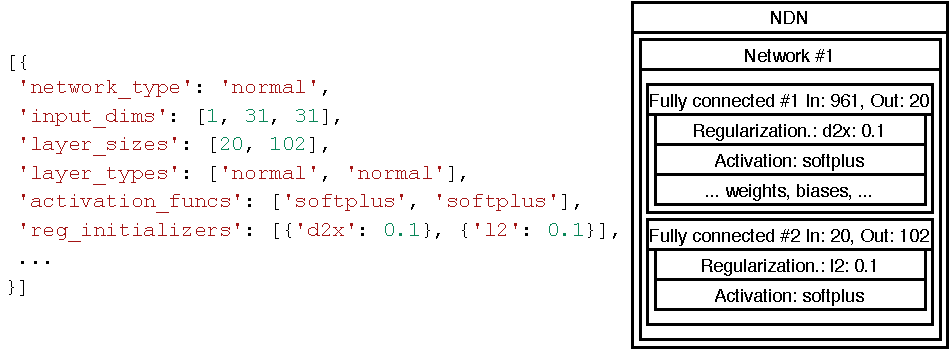
\includegraphics[width=1\textwidth]{../figures/03_NDN_1}
    \caption[NDN model description and subsequent architecture]{Model description and the resulting NDN instance for an LNLN model with 31x31 pixels input, 102 output neurons, 20 filters, SoftPlus non-linearities, and regularizations.}
    \label{fig:3.1}
\end{figure}

The NDN model class recursively contains instances representing its parts. The NDN object includes an array of network objects, each network object contains a stack of layer objects, and each layer object has, among others, regularization objects. The layer object also contains fields representing all of its hyperparameters, specifying its activation function, and - among a few more - also maintains NP arrays backing all its free parameters such as weights and biases. All of this structure is created as part of the network's definition which happens from within the NDN’s constructor. This is also where parameters initialization happens through the backing NP arrays.

Whenever computation is invoked - e.g. when \texttt{train} or \texttt{generate\_predic\-tion} methods are called, a new TF session is initialized, a computational graph is recursively created from scratch using the description saved on the internal network and layer objects, and finally, weights are loaded to the session from the aforementioned layers’ parameters backing NP arrays. When the computation finishes, all weights are gathered from the TF session to plain NP arrays and saved within layers’ objects of the model again. For visualisation, refer to figure \ref{fig:3.2}.

All shapes are inferred from input dimensions, specified layer sizes, and - e.g. in the case of convolutional layer - its stride and filter size, with the last layer size serving as the output dimensions. The interpretation of input dimensions is (\texttt{time}\footnote{This is to support temporal models which we will not cover.}, \texttt{width}, \texttt{height}). Internally, the framework assumes \texttt{(batch\_shape, height, width, channels} or \texttt{time)} dimensionality and uses flatten representation to float data between layers. When necessary, for example to apply 2D convolution, a layer restores the full dimensionality, both spatial and channels/time dimensions, and, after applying its function, flattens the data again. 

\begin{figure}[ht]
    \centering
    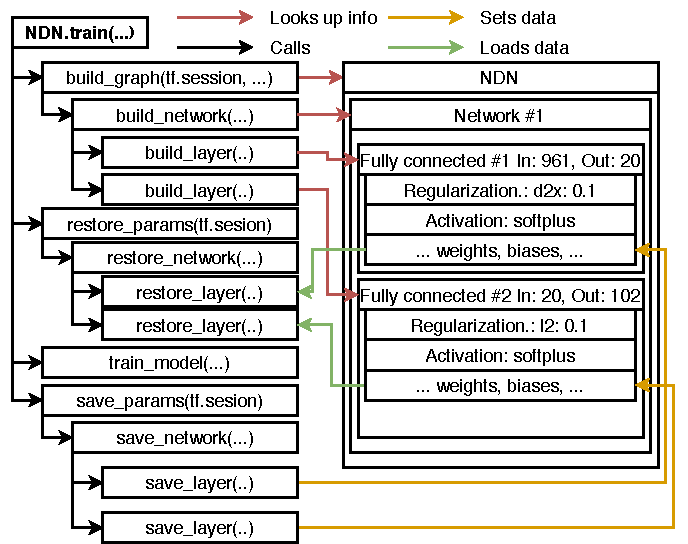
\includegraphics[]{../figures/03_NDN_2}
    \caption[NDN computation graph initialization]{Diagram of NDN model initialization when \texttt{train(...)} method is called.}
    \label{fig:3.2}
\end{figure}

\subsection{NDN3 toolkit}\label{ch:3.1.1}

The featureset of NDN3 is vast and continuously evolving and so it is not our intention to provide a comprehensive summary. Below is just a subset of tools that are either relevant to our work (implemented additions in \textit{italic}) or that we wanted to particularly draw attention to for potential future continuation of our exploration.

\begin{itemize}
    \item \textbf{Loss functions (noise assumptions):} Gaussian, Poisson, Bernoulli.
    
    \item \textbf{Layers:} Fully connected (normal), Separable, Convolution, Convolutional separable\footnote{Each filter is factored into a convolutional \textit{what} and \textit{where} masks.}, Readout\footnote{Outputs the value of spatial location defined by an explicit parameter. Not to be confused with general \textit{readout layer} (any first layer after convolutional layers).}, Convolutional readout, Additive\footnote{Combines inputs from multiple input streams.}, \textit{DoG}, \textit{Convolutional DoG}, \textit{Linear scale}\footnote{Linearly scales its input using a scalar multiplier and single additive bias: $input*x + b$.}, etc.
    
    \item \textbf{Parameters regularizations\footnote{Regularizations are the only externally documented part of NDN: \href{https://github.com/NeuroTheoryUMD/NDN/blob/master/docs/glossary.rst}{https://github.com{\-}/NeuroTheoryUMD/NDN/blob/master/docs/glossary.rst}}:} Dropout, center\footnote{Penalizes higher weights far from the center.}, norm2\footnote{Encourages norm of weight matrix to be 1.}, max\footnote{Penalizes each pair of non-zero weights (i.e. heavily discourages more than 1 non-zero weight), both in spatial and channel dimensions.}, L1, L2, Spatial Laplacian (d2x), etc.
    
    \item \textbf{Parameters normalizations\footnote{This is parameters normalization i.e weights are normalised each time before used. Activation normalization, such as batch normalisation \citep{2015arXiv150203167I}, is notably missing.}:} maxnorm, L2.
    
    \item \textbf{Activation functions:} ReLU, sigmoid, tanh, identity, SoftPlus, leaky ReLU, etc.
    
    \item \textbf{Weights/bias initializers:} zeroes, normal\footnote{Normal distribution with 0 mean, 0.1 variance.}, trunc normal\footnote{Absolute value of normal.}.
\end{itemize}

Apart from these traditional tools, NDN3 also provides following capabilities:

\begin{itemize}
    \item \textbf{Metrics capture:} Loss value and \textit{potentially\footnote{Not merged upstream, please refer to the \tttnameref{at:msc-neuro}'s \texttt{./README.md}.} correlation metrics} can be logged as TF summaries periodically throughout the training loop as part of the summary step.
    
    \item \textbf{Layer activation logging:}  In addition to model-wide metrics such as the loss value, NDN3 allows for individual layers’ activations to be logged as histograms.
    
    \item \textbf{Validation while training:} If specified, a validation set can be evaluated using abovementioned metrics as part of the summary step of the training loop every few epochs. Do note that the validation set is evaluated in its entirety at once and is not batched. Respective metrics are saved as a separate TF summary.
    
    \item \textbf{Support for early stopping:} Using the same mechanism as the abovementioned validation metrics, NDN3 supports early stopping.
    
    \item \textbf{Explicit inhibitory/excitatory neurons enforcement:} It is possible to specify the ratio of excitatory/inhibitory neurons on supported layer types (normal, convolution, etc.). This works through enforcing strictly non-negative weights and then multiplying the layer’s output with a +/-1 mask.
    
    \item \textbf{Data filters:} In addition to input and output data, it is possible to provide data filters. A boolean mask of the same dimensionality as the output data that specifies which individual output neurons should be ignored (zeroed for prediction, ignored for loss value computation, metrics, etc.) for what particular data points. This allows for, among other things, a common model trained on two separate recordings (e.g. 10 and 15 data examples) of two neuron regions (e.g. containing 5 and 7 neurons). The output dimensionality of such a model would be 12. Where valid output data are not available, i.e. for neurons 5 to 12 of the first 10 data points, zeroes can be used. In such case, the data filter mask has ones on the indexes 0 to 5 for the first 10 data points, and zeros for indexes 5 to 12. The situation is mirrored for data points 10 to 25. This way, when NDN model computes an output of a second region’s neuron (e.g. neuron 11) for a first region’s data point (e.g. 5th data instance) while training, it can see the 0 in \texttt{data\_filters[5][11]} mask and know to not include its not-trained output in the loss function computation and subsequent optimisation.
    
    \item \textbf{Many more:} Several data ingestion pipelines, support for temporal models, etc.
\end{itemize}

\section{Implemented NDN3 extensions}\label{ch:3.2}

To facilitate our research, we implemented several extensions to the NDN3 framework\footnote{Most additions were merged upstream but some remain only in a fork (attachment \ref{at:ndn3}). For more information, refer to \tttnameref{at:msc-neuro}'s \texttt{./README.md}.}. Our main contribution was in the form of the Difference of Gaussians layer\footnote{For description, refer to \refsection{ch:2.1.1}.} as introduced by \cite{antolik}. We also implemented a convolutional variant of this layer. To help with training progression interpretability, support for Pearson’s correlation tracking as part of TF summary was also added, as well as several general fixes and other smaller-scale contributions.

\subsection{DoG layer \& convolutional variant}
The Difference of Gaussians (DoG) layer is implemented similarly to a fully connected layer, with two main differences. Instead of input dimensions worth of weights per each output neuron, it only has 6\footnote{It actually reserves 8 to support not-concentric difference-of-Gaussians filters. Such behavior is off by default but can be enabled through \texttt{impl\_concentric} parameter.}. And instead of using these weights directly, only reshaped, to multiply the input with, they are used to create a full difference-of-Gaussians filter first. Namely, they are separated into the shared center x, y coordinates, and weights and diameters parameters for each of the Gaussians. Then, the full gaussian filter is computed\footnote{This is likely not the most efficient implementation but given the size of our data and other bottlenecks within the system it never showed to be an issue.} with dimensionality of \texttt{(input\_width, input\_height, 1, number\_of\_channels)}, element-wise multiplied with the layer’s input, and spatially sum-reduced, creating a \texttt{number\_of\_channels}-wide output tensor. The output is then normally processed through activation function, bias, dropout, etc.

The convolutional DoG variant works similarly, the only two differences being the size of the difference-of-Gaussians filter and its application. The filter is of size \texttt{conv\_filter\_widths} and, rather than being pointwise multiplied with the input, it is applied at all of its spatial locations as per the semantics of conv2D operation\footnote{\href{https://www.tensorflow.org/api_docs/python/tf/nn/conv2d}{https://www.tensorflow.org/api\_docs/python/tf/nn/conv2d}}. The same as a classical convolutional layer, it supports convolution stride and dilations. The \texttt{SAME} option is used for padding. 

Unlike the weights of fully connected and convolutional layers or their direct derivatives, the weights of either classical or convolutional variant of DoG cannot be initialized using the mechanisms already provided by NDN3\footnote{Refer to \refsection{ch:3.1.1}.}. Namely, the Gaussians center(s) needs to fit within the spatial boundaries of the input/convolutional filter, and the width should at least be proportional to the spatial dimensionality. Given that, we opted for replicating the exact initialization scheme of \citeauthor{antolik}, drawing the DoG parameters from a uniform distribution with bounds proportional to the input/convolution filter size. Namely, the weights are strictly positive, widths are bounded by 1 pixel and 82 \% of the maximum of input/filter width and height, and the center cannot be closer to an edge than two pixels. 

\subsection{Pearson's correlation tracking}
The Pearson's correlation tracking is implemented as part of the loss function evaluation. It is computed for each output neuron separately and then averaged. Several options are available: interpreting neurons’ NaN correlations as 0, ignoring NaN correlations, and - inspired by \cite{ecker} - also ignoring correlations for neurons with small variation in the recorded data. All of our experiments use the \texttt{treat NaNs as zeroes} option. The correlation tracking respects data filters\footnote{Refer to \refsection{ch:3.1.1}.} if set, properly ignoring outputs of masked neurons.

\section{Experiments and analysis pipeline}\label{ch:3.3}

To enable scalable execution and evaluation of a large number of architectures implemented using NDN3, including the capability for efficient hyperparameter search, we also created\footnote{The code is hosted together with all experiments in \refattachment{at:msc-neuro}.} an experiments and evaluation pipeline. It consists of three parts, experiment execution pipeline, results and analysis tools, and general NDN3 utils.

\subsection{Experiment execution}
The experiment execution pipeline works as follows. For each experiment, two python scripts exist, a \textit{runner} and the \textit{experiment} itself. The \textit{runner} iterates over all hyperparameter combinations the experiment is supposed to test and calls the experiment script with each of the combinations as command-line arguments. It does not call it directly, however, but through a backend-specific \textit{executors}. The one to be used is user-selected when the runner script is invoked. Currently, five backend \textit{executors} are implemented, one for a custom Docker-based\footnote{https://www.docker.com/} environment, two for qsub\footnote{https://en.wikipedia.org/wiki/Qsub} based systems - CPU and GPU version, and two for plain virtenv python environments on windows or linux. For each of them, separate \textit{experiment script} invocations are either submitted as individual jobs or are natively run in parallel. All of them redirect standard output and standard error to by-convention-standardized log files.

\begin{figure}[ht]
    \centering
    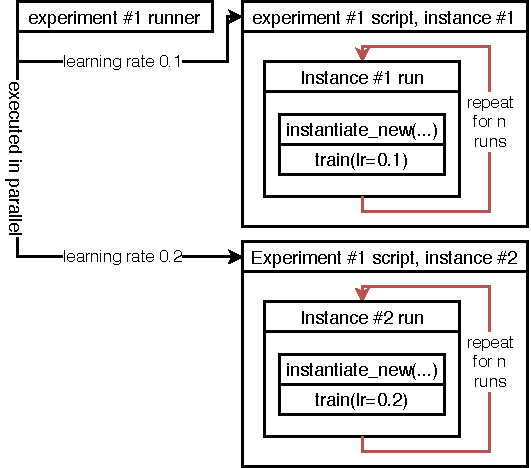
\includegraphics[]{../figures/03_msc-neuro_1}
    \caption[Experiments pipeline]{Experiments pipeline: Execution order when an \texttt{experiment \#1} with two instances (learning rate 0.1 and 0.2) is run through a runner.}
    \label{fig:3.3}
\end{figure}

The \textit{experiment script} can be arbitrary, but - by convention - contains instantiation and training of a specific model architecture given a particular set of (hyper)parameters (further referred to as the \textit{experiment instance}) passed as command-line arguments, usually by the corresponding \textit{runner}. As further explained in \refsection{ch:4.2.1}, each model instance is actually instantiated and trained multiple times (further referred to as the \textit{experiment instance run}) to control for the influence of random initialization. Currently, for all implemented experiments individual \textit{instance runs} are executed sequentially by the respective \textit{experiment scripts}. For illustration, refer to figure \ref{fig:3.3}.

\subsection{Experiment analysis}
Having multiple \textit{runs} of, apart from random initialization, identical models pre\-sents a challenge for analysis. Instead of comparing performance of individual \textit{runs}, sets of multiple \textit{runs} need to be considered. To facilitate that, an analysis toolkit was created. A user can specify a list of \textit{experiment instances} to be compared against each other as an array of root folders with TF summaries and filter regexes. Based on that, all relevant TF summaries of each \textit{experiment instance} are gathered. For each \textit{instance}, metrics are first read from the summaries files of all \textit{runs}, then the values grouped by epoch number (step), and finally a few general statistics, such as deciles of performance, are computed across each \textit{instance}’s individual \textit{runs}. As the last step, the results are presented either as a graph (see figure \ref{fig:3.4}) - showing the metric percentiles of each \textit{instance} in time, or as a summary table - representing the final trained performance. 

\begin{figure}[ht]
    \centering
    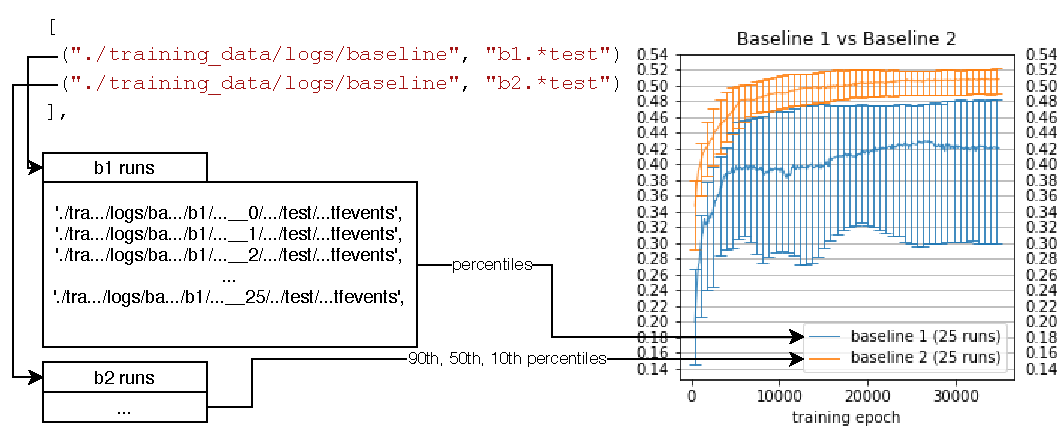
\includegraphics[width=1\textwidth]{../figures/03_msc-neuro_2}
    \caption[Experiment analysis toolkit]{Experiment analysis toolkit: Retrieval of summaries for individual runs of two experiment instances (\texttt{b1}, \texttt{b2}).}
    \label{fig:3.4}
\end{figure}

For more information about the specifics, such as the expected filesystem layout of the experiments pipeline or the exact API of analysis toolkit, please consult either the \tttnameref{at:msc-neuro}’s \texttt{./README.md} or the documentation that is part of respective methods’ source code. 
